\documentclass[12pt,a4paper]{report}
\usepackage{hyperref}
\usepackage{graphicx}
\usepackage{wrapfig}
\usepackage{pdfpages}
\usepackage{subfigure}

\graphicspath{{images/}}
\pagenumbering{arabic}

\AtBeginDocument{\renewcommand{\bibname}{References}}

\begin{document}

\begin{titlepage}
  \centering
  {\scshape\LARGE University College Cork \par}
  \vspace{1cm}
  {\scshape\Large Department of Computer Science\par}
  {\scshape\Large Final year project BSc in Computer Science\par}
  \vspace{1.5cm}
  {\huge\bfseries Word of the People\par}
  \vspace{2cm}
  {\Large\itshape Conor Tak Saruwatari\par}
  \vfill
  supervised by\par
  Dr.~James \textsc{Doherty}

  \vfill

% Bottom of the page
  {\large April, 2017\par}

\end{titlepage}
{\scshape\LARGE Declaration of Originality \par}
  \vspace{1cm}
  In signing this declaration, you are conforming, in writing, that the submitted work is entirely your own original work, except where clearly attributed otherwise, and that it has not been submitted partly or wholly for any other educational award.
  \linebreak
  I hereby declate that: 
  \begin{itemize}
    \item this is all my own work, unless clearly indicated otherwise, with full and proper accreditation;
    \item with respect to my own work: none of it has been submitted at any educational institution contributing in any way to an educational award;
    \item with respect to another’s work: all text, diagrams, code, or ideas, whether verbatim, paraphrased or otherwise modified or adapted, have been duly attributed to the source in a scholarly manner, whether from books, papers, lecture notes or any other student’s work, whether published or unpublished, electronically or in print.
  \end{itemize}
  Signed: . . . . . . . . . . . . . . . . . . . . . . . . . 
  \linebreak
  Date: . . . . . . . . . . . . . . . . . . . . . . . . . . . . . . . . . . . . . . . . . . .



\begin{abstract}
  In the current age Twitter has wuickly become one of the most popular forms of Social Media. Its fast pace and the concise nature of its 140 character limit make it an invaluable source of information into the opinions and stance of a massive population. The goal of this project is to create an efficient means of analyzing and compiling this data in an effective manner such that it can be used for market research, recommender systems, predictive AI and any other number of possible applications. This was developed in Python while restricting available resources to those legally usable within corporate development, such as libraries holding an MIT Software License.
\end{abstract}

\tableofcontents

\listoffigures

\chapter{Introduction}
  Since 2007, Twitter has quickly risen to become one of the most popular forms of Social Media. Its fast pace and 140 character limit provide quick, concise opinions on a wide variety of topics. This makes it an invaluable source of information into the opinions and stances of a massive population.
  \par
  Development was handled almost entirely in Python 2.7\cite{Python2Docs} and use of extra libraries was restricted to those usable within industrial or corporate development environments, such as those with an MIT License\cite{MITLicense}.
  \section{Motivation}
    While working as a Software Engineer at IBM\cite{IBM} as part of my Work Placement during the summer of 2016 I spent a lot of time working with large amounts of data. Compiling and aggregating large volumes of raw data into usable reports and logical conclusions. I found this work both interesting and engaging, leaving me with a desire to continue into such analytics after my placement concluded. This project has given me the opportunity to explore this subject matter further, deepening and enhancing my own knowledge and experience in data handling and analysis.
    \par
    Even after my work at IBM, I knew I had only just scratched the surface of big data analytics. I had mapped reports and diagnostics to hard coded conclusions but I had done very little work into analyzing specific elements of the data itself. Feeling both confident in my ability I figured text analysis would be an interesting topic to explore. However, knowing very little of the analysis of abstract data I decided to work with smaller individual items on a larger scale so as to keep the analysis itself simpler to implement and run. This led me to working with Tweets.
    \par
    The learning curve as I embarked on the project was far from lenient. At several points considerably steeper than previous work I had undertaken. My previous knowledge of Python did not cater for the scale of this work and my knowledge of raw text analysis was, at the time non-existent. Throughout development I have learnt everything necessary about these subjects and how they can be applied to accurate Text Analysis.
  \section{Goals}
    The primary goal of the project was to build a program capable of simultaneously running efficient and effective data collection and analysis while also capable of compiling all previously assessed data for analysis and aggregation on demand. This data was to be highly generalized, easily readable for both human users and predictive analysis. 
  

\chapter{Analysis}
  \section{Objectives}
    The main objective of the project is to create an effective and efficient text analysis, capable of being performed in real time for any variety of uses, from market research to predictive analysis. The analysis was kept generalized as topical language development would have taken a much greater length of time. For example if searching for opinions on a horror movie, words such as terrifying and gory would be positive, however in a generalised case these would be counted as negative opinions. As such the idea of topical text analysis was dropped before development even began. 
    \par
    Scalability was a topic discussed often while I was working at IBM. To ensure ease of scaling and parallelization I developed the project exclusively on my own laptop. As such some later basic shortcomings and limits in processing speed could be compensated in a higher level implementation. However the basic implementation on the laptop had to function effectively as a proof of concept.

\chapter{Design}
  The final version of the project was composed of 6 main modules to run. The main command line interface WOPMain.py\cite{SourceCode}, the text cleaner textClean.py\cite{SourceCode}, the text analyzer textAnalysis.py\cite{SourceCode}, the tweet handler tweetHandler.py\cite{SourceCode}, the tweet scraper twitterScraper.py\cite{SourceCode} and a database class MyDB.py\cite{SourceCode}.
  \section{Main Interface}
  Once the main interface is started it gets the details of all current clients from the database. Within the database ‘clients’ are stored as strings used to scrape data, coupled with a rate in seconds between data collection and a count of tweets per collection. For each client a thread is created that waits for the specified seconds before attempting to collect data from Twitter. An entry is also made into the log on the initialisation of thread as well as the current wait time. All Threads share a single database interface and will attempt to complete their wait between Twitter calls if the main is shut down. Each thread independently requests, analyzes and stores tweets until the main is closed.
  \section{Text Cleaner}
  The text cleaner was designed to act as an early level filter for the project. It was designed to clear away links as well as irrelevant tweets. Tweets wherein links made up more than half of the text were dropped before analysis took place. Initially this was supposed to make use of Twitter entities, however due to an issue in gathering older testing data and the project’s workaround, this functionality was abandoned.
  \section{Twitter Scraper}
  The scraper handles all calls to the official Twitter API. Initially it was built using the TwitterSearch\cite{TwitterSearch} library, however this library led to several issues late in development when threading was being implemented. To resolve this problem development was moved to the Twython\cite{Twython} Library. Both of these libraries were officially licensed by Twitter. Twitter’s API consistently caused issues throughout development due to a number of factors which will be covered in Evaluation, see Page \ref{eval}.
  \section{Twitter Handler}
  The handler was built to parse the key information from Twitter API calls. It was initially created early on in development however it was then dropped from the project and rebuilt towards the end of development. Each individual tweet was comprised of roughly 200 lines of different JSON values, some of which were depreciated so parsing the key details and reducing raw data flow was a key part of the overall process.
  \section{Text Analyzer}
  The text analyzer was one of the two main focuses of the project. It was specially designed for Twitter, using small features such as emojis and hashtags to build a more accurate, in-depth analysis. One of the most important aspects of this process, however was to streamline it as a real world implementation would likely deal with hundreds of thousands of tweets per minute. At the time of this report the average analysis time for the text of a tweets took less than a ten thousandth of a second.
  \section{Database}
  The database class was built using Object Oriented Python to encapsulate all Database functionality for the project. Initially I had planned on developing the project around a MongoDB\cite{MongoDB} database due to the JSON dictionary structure of tweet information. However as development moved ahead the data became more reduced and concise, lending itself more to a MySQL\cite{MySQL} implementation than that of MongoDB. The class was used for all database interaction, from simple data request to aggregating tweet information for graphing.

\clearpage
\chapter{Implementation}
  \section{Project Planning}
  \begin{figure}[h]
  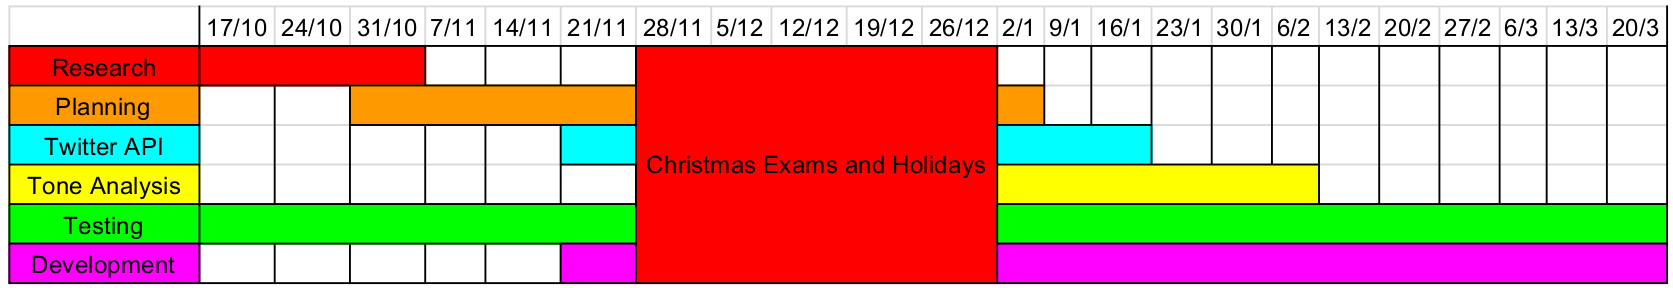
\includegraphics[width=\textwidth]{tt1}
  \caption{First Gantt Chart Draft}
  \label{fig:tt1}
  \end{figure}
  Project Planning began immediately after the project brief was accepted in October. As can be seen above \ref{fig:tt1} there an initial estimate of 6 weeks necessary for research and planning. With work to begin with the Twitter API towards the end of the sixth week. A five week period from the end of November through December was set aside to allow time for the Christmas Exams as well as the Christmas break. Work on interfacing with the API was to resume immediately after New Years and work on the text analysis was to begin around the same time. Testing on various small project elements was to take place throughout development from assessing Python Libraries for Twitter to resting more efficient means of Text Analysis.
  \par
  \begin{figure}[h]
  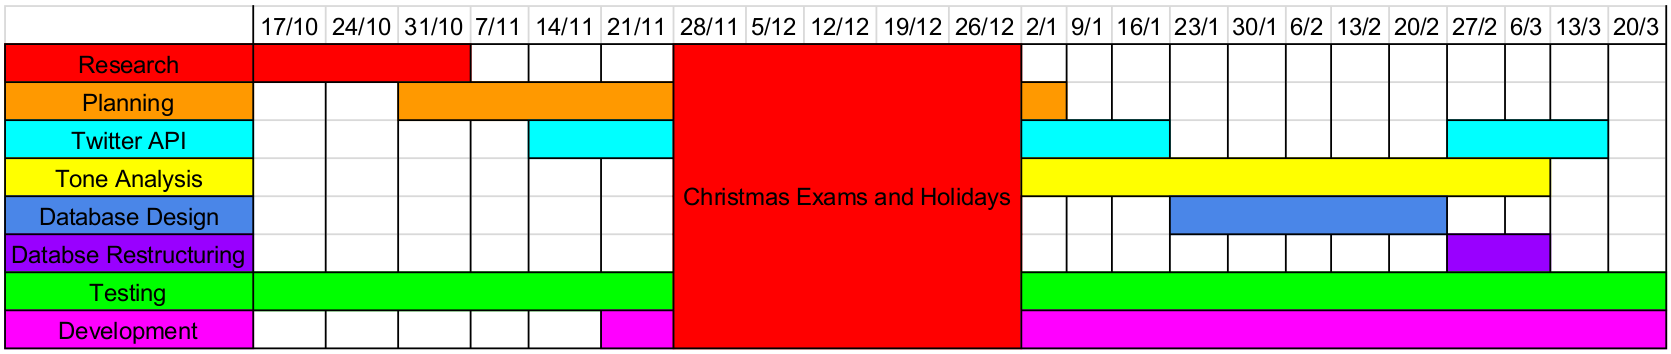
\includegraphics[width=\textwidth]{tt2}
  \caption{Final Gantt Chart Draft}
  \label{fig:tt2}
  \end{figure}
  As is often the case in any planned project, the initial plan was the first thing to go. Early Twitter API test went so well I began work on a Python interface a week earlier than planned. After Christmas I managed to finish up work on my TwitterSearch\cite{TwitterSearch} wrapper module and began work on the Text Analysis. Before Christmas I had done research into different Text Analysis Software such as Natural Language Toolkit or NLTK\ref{NTLK} and began with a simple unweighted words scan. Comparing words to items in predetermined .txt files containing positive and negative words. It was slow and clunky, but functional. Satisfied for now I began planning the Database Structure.
  \clearpage
  \section{Disecting Tweet Structure}
  Early work in development began by dumping collected tweets in a JSON\cite{JSON} file. Each tweet consisted of nearly 200 different tags and values. As a result parsing the usable information from the structure proved to be difficult as large amounts of data were repeated. Furthermore several of the tags used were depreciated and served no purpose whatsoever. 
  \section{Database Structuting}
  \begin{wrapfigure}{r}{0.75\textwidth}
    \centering
    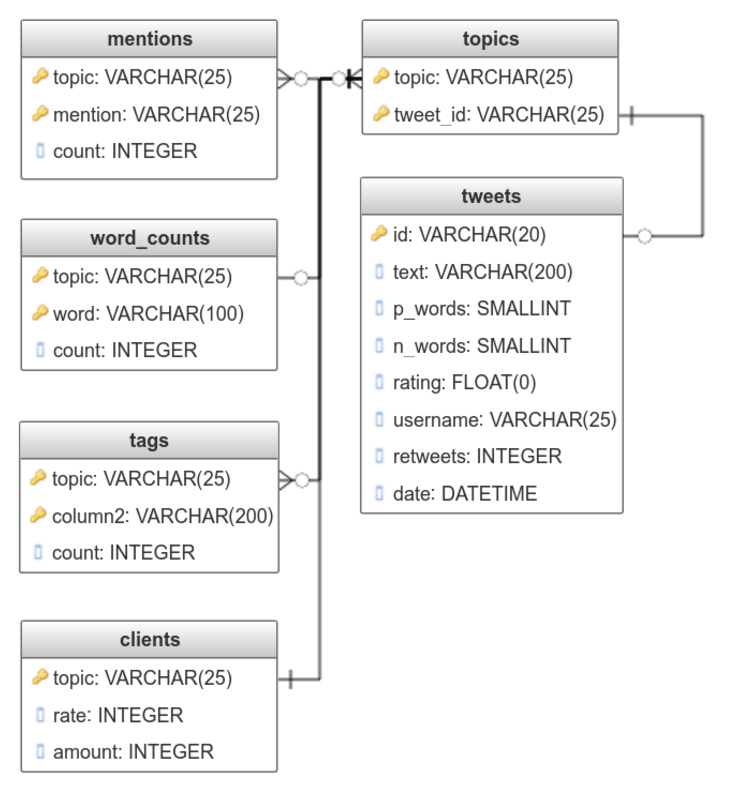
\includegraphics[width=0.75\textwidth]{dber}
    \caption{Finalized Database Schema}
    \label{fig:dber}
  \end{wrapfigure}
  Due to the JSON\cite{JSON} structure of the tweets I initially began implementing a MongoDB database on a topic by topic basis. However as I began giving more thought to the overall database structure and how best to minimize cost while maximizing usable data and reducing data aggregation complexity I realised that I had simplified by data to the extent that it could be reduced to a more cost effective MySQL database.
  \clearpage
  \section{Test Data Collection}
  Following the database restructuring I continued work on the Text Analysis, however I found myself lacking in ideas for usable topics and data. In the end I decided to build a several large collections of Tweets from the previous 3 U.S. Presidential Elections. I ran a request through the official API but discovered that it limited returned Tweets to those less than a week old. I began research and found an unofficial library that scraped data directly from the Twitter Advanced Search Browser API. I began with a quick collection of ten thousand tweets from the thirty days prior to the actual election day for each candidate. (Barack Obama twice). At the suggestion of a fellow student I also pulled tweets on Sarah Palin for the 2008 U.S. Presidential Election as she was just as large a point of discussion as John McCain. This process ultimately left me with about sixty thousand tweets. However, disappointed in the variety of data I wrote a small script to pull up to ten thousand tweets from each day up to thirty one days prior to the actual election. 
  \par
  This process ultimately led to several complications. The largest of which was a combination of Twitter’s API and the unofficial Python library. As I was making multiple requests to the API for large volumes of data, if I made too many my access to the API would be suspended by Twitter. Secondly the library was designed such that if a request to the API was rejected it would exit Python, breaking any loop in which I attempted use for the process. Ultimately I changed the library myself to remove this feature and successfully created a functional script. The script left an hour wait in between API calls as well as in the event of an API rejection. After a little under two weeks and minimal API rejections I finally had a satisfactory testing dataset.
  \clearpage
  \section{Text Analysis}
  \begin{figure}[!htb]
    \centering
    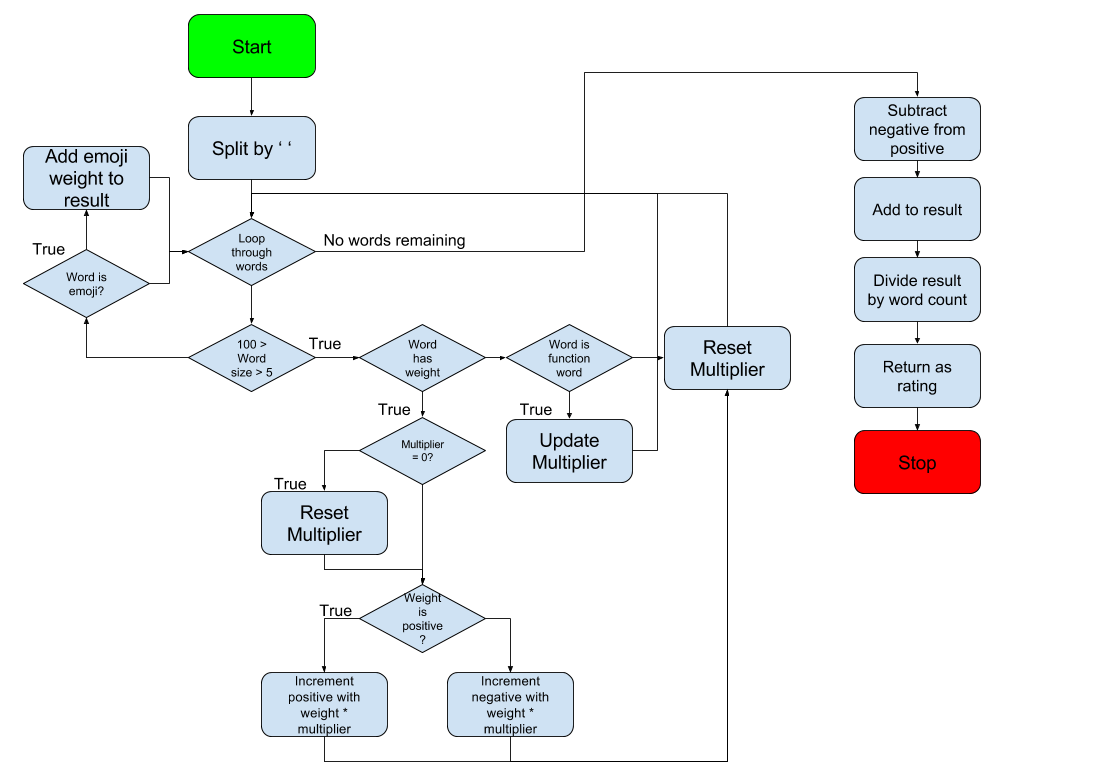
\includegraphics[width=\textwidth]{textAnalysis}
    \caption{Simplified Text Analysis Process}
    \label{fig:activityDiagram}
  \end{figure}
  While I ran the data collection script I began enhancing the Text Analysis, allowing for functional words to invert, enhance or detract from the weight a word had on the overall rating of a tweet. These function words also affected each other but the weight would be ignored if a positive or negative word did not follow them. Hashtags were also added as a means of emphasis on whatever word they were used and mentions were catalogued to allow for analysis of individual users. As a final addition a small library of emojis were added to the analysis. Ultimately the greatest enhancement to the text analysis came in the form of a small fix. Throughout most of development words were stored in a list with a linear search through each list used to inform the program of a word’s classification.  
  \par
  Following most of my work on the Text Analysis I began working on a means of interacting with and controlling the software. I began with a small and basic interface that ran each ‘client’ in a queue. However this implementation was incredibly inefficient so I began working on running each ‘client’ on individual Threads, something I had never dealt with in Python. This took a little over a week to finalize and hit multiple setbacks during implementation. One of the first issues was in safely shutting down the interface. Due to the delay in client request, (rate in the database table) the interface itself could not shut down until the delay had completed for all Threads. A larger problem however, was an issue surrounding the TwitterSearch\cite{TwitterSearch} Python library, which had been causing a series of errors with the Threads, ultimately preventing any Threads from successfully starting. To resolve this issue I abandoned the TwitterSearch\cite{TwitterSearch} library for the Twython\cite{Twython} library which thankfully ran smoothly when added to the threaded implementation.
  \par
  Most of the later development on the Interface was carried out in tandem with later database development. As multiple UI features were added to simplify the interface for a generalized user as well as several commands for data aggregation and display. Some of this more complicated data compilation did prove to be the larger of issues within the final stages of development

\chapter{Evaluation}
\label{eval}
  Overall, I am unsatisfied with how my project ended up. There are many elements I would have loved to have gotten the opportunity to refine further which I may ultimately end up doing in my own spare time.
  \section{Weights}
  \begin{wrapfigure}{r}{0.2\textwidth}
    \[rating \times \frac{retweets}{avg(retweets)}\]
    \caption{Current Weight Function}
  \end{wrapfigure}
  At present there is a bare minimum weight function built into the interface that weighs the overall rating of a tweet based on its retweets in comparison to the daily or hourly average, depending on data grouping.
  \par
  \begin{figure}[h]
    \centering
    \subfigure[Weighted Hourly Data]{
      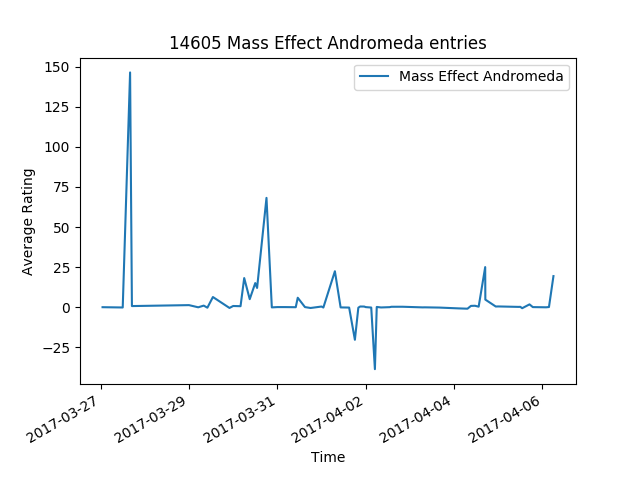
\includegraphics[width=0.3\textwidth]{mea_h_w}
      \label{fig:hwd}
    }
    \subfigure[Unweighted Hourly Data]{
      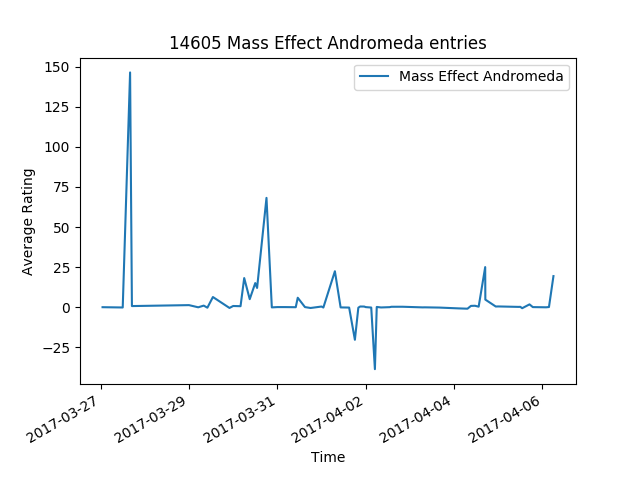
\includegraphics[width=0.3\textwidth]{mea_h_w}
      \label{fig:hud}
    }
    \subfigure[Unweighted Daily Data]{
      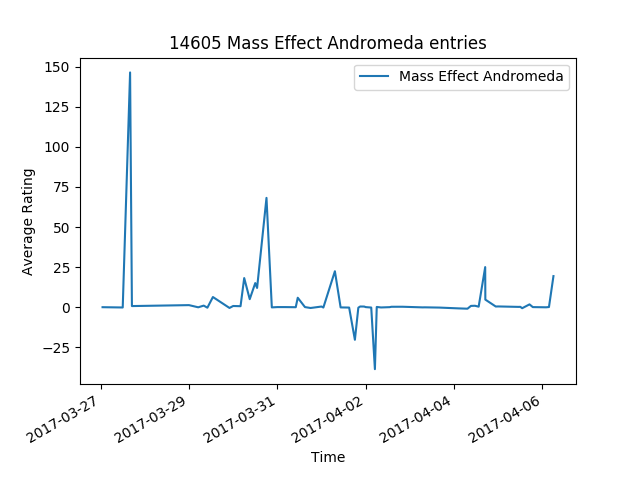
\includegraphics[width=0.3\textwidth]{mea_h_w}
      \label{fig:dud}
    }
    \caption{Graphed Data}
    \label{fig:gd}
  \end{figure}
  Unfortunately due to the low volume retweets on the majority of database entries the resultant value becomes $\approx$ 0, resulting in the data being ignored. As shown in Figure \ref{fig:hwd} as opposed to Figure \ref{fig:hud}. I attempted to get some data to show the comparison at a daily scale, however when weighted there was no available data as opposed to the unweighted data in Figure \ref{fig:dud}.
  \par
  In the end the function removed most available data for any given topic with most tweets falling far below this average. Given more time and further development it would have been interesting to look into a more accurate and in-depth means of weighing these tweets for data compilation. However at present a concrete implementation for doing so escapes me.
  \section{Data Collection}
  As a proof of concept I decided early on to test the text analysis on previous U.S. Presidential Elections. however as discussed in Implementation. This proved to be one of the most time consuming and tedious points in development. As discussed in Implementation.
    \subsection{Twitter Itself}
    Throughout development Twitter itself proved to be the largest bottleneck. The official API only allows access to data less than a week old and limits individual request to 100 individual tweets. On top of this there are additional limits on how many request can be made from a developer and/or IP address\cite{TwitterAPILimits}. One of the largest delays in the project’s overall development was the time spent collecting data from the 2008, 2012 and 2016 elections as I had to use an unofficial library to scrape the data. This was both inefficient and was contrary to one of my open source development restriction. However I ignored this as the library itself used an MIT License\cite{MITLicense} and was not a part of the final project. 
    \subsection{Altered Library}
    During Data Collection I had to alter the code of this library myself. This was to allow for pausing of the collection script in the event of an API rejection. The data I received from this library was also inefficient as it lacked many of the more specialised tags included in officially retrieved twitter data, such as the entities tags which would have allowed for faster retrieval of mentions, hashtags and most importantly links. Due to this limitation I was forced to greatly reduce the planned functionality of the text cleaning module. I had initially planned on having the module access the link and replace the link with the title of the web page within the text body of the tweet.
  \section{Unimplemented Features}
  Due to a number of factors, some mentioned previously as well as others such as time there were a number of features that I was unfortunately unable to implement.
    \subsection{Topical word collections}
    As mentioned in Analysis in the example of a horror movie, words such as terrifying and gory would be considered positive attributes. However in the current generalized case these would qualify as negative opinions leading to an inaccurate analysis of a topic.
    \subsection{Twitter Entities}
    The finalized text analysis, at the time of this report was built around the data acquired from the aforementioned third party analysis. Unfortunately the data returned by this library was heavily simplified and lacked one of the most useful of Twitter's API features; entitities\cite{TwitterEntities}. Entities isolted and reference many of the useful pieces of information in a tweet. i.e. tags, mentions and most importantly media and urls. I had planned to use these entities to remove and record mentions prior to text analysis. Furthermore I had planned on replacing links in text with the HTML title of whatever the link approached by means of automated HTTP requests and Web scraping.
    \par
    Unfortunately the data scraped from Twitter lacked these entities and this functionality was unfortunately abandoned for an ineffective link scanner. Mention scanning was built into the text analysis and urls were left unused despite being the main focus of a large portion of all tweets.
  \par
  Looking back over the project now, were I to do the project all over again I definitely would have looked into more Twitter libraries, or created my own means of scraping the data so that I would be far less limited by the official Twitter APIs.

\chapter{Conclusions}
  In conclusion I am dissatisfied with my finalized project. The url scanning is ineffective and is not being used to better reflect the opinions of users. Admittedly doing so would ultimately greatly increase the scan time of tweets, however my unimplemented method would replace links within the body of a tweet, at minimum removing this overhead for a database rescan.
  \section{Data Analysis}
  \begin{figure}[h]
    \centering
    \subfigure[U.S. Presidential Election 2008]{
      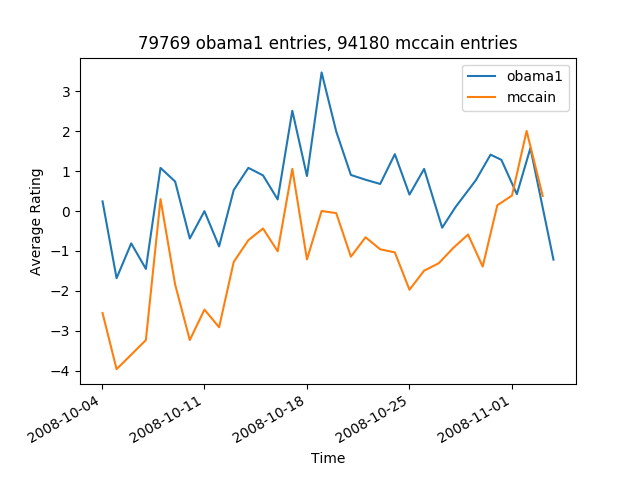
\includegraphics[width=0.3\textwidth]{e1}
      \label{fig:e1}
    }
    \subfigure[U.S. Presidential Election 2012]{
      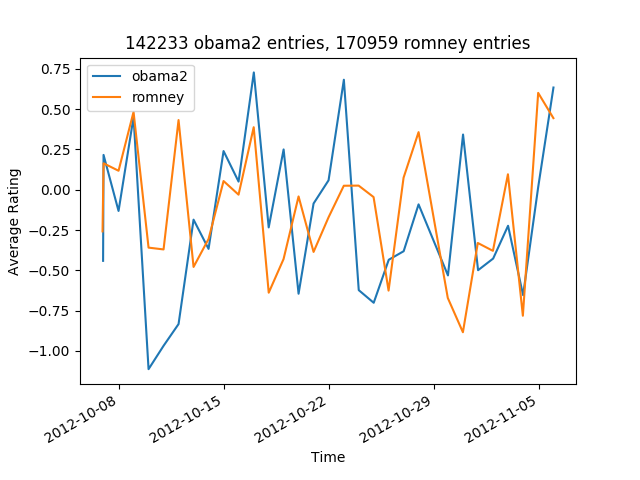
\includegraphics[width=0.3\textwidth]{e2}
      \label{fig:e2}
    }
    \subfigure[U.S. Presidential Election 2016]{
      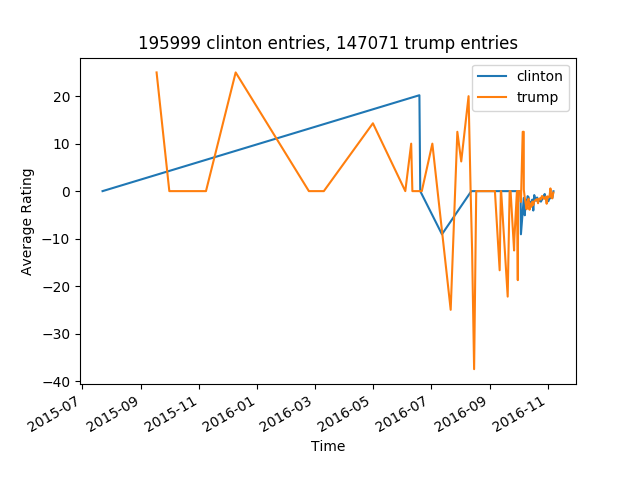
\includegraphics[width=0.3\textwidth]{e3}
      \label{fig:e3}
    }
    \caption{Graphed Presidential Elections}
    \label{fig:ex}
  \end{figure}
  As shown above in Figure \ref{fig:ex} the finalized analysis was reasonably usable, however the finalized states of the topics shown in Figure\ref{t:1} show that the accuracy of the analysis could still be greatly improved upon.
  \begin{figure}[h]
    \centering
    \begin{tabular}{|c||c|c|c|c|}
      \hline
      \multicolumn{5}{|c|}{Topic States} \\
      \hline
      Topic & Tweets & Average Rating & Average Positive Words & Average Negative Words \\ [0.5ex]
      \hline
      \hline
      obama1 & 79769 & 0.5948484 & 0.3468 & 0.3197 \\
      \hline
      mccain & 94180 & -0.9966915 & 0.3021 & 0.3751 \\
      \hline
      obama2 & 141969 & -0.19368869 & 0.2544 & 0.2766 \\
      \hline
      romney & 170644 & -0.12087439 & 0.2529 & 0.2648 \\
      \hline
      clinton & 194749 & -1.74210266 & 0.1954 & 0.3328 \\
      \hline
      trump & 146729 & -1.886695064 & 0.2527 & 0.3848 \\
      \hline
    \end{tabular}
    \caption{Final State for Collected Election Data}
    \label{t:1}
  \end{figure}
  \section{Efficiency}
  Efficiency of execution is one of the few categories with which I am satisfied with my project in its current state. As shown below in Figure \ref{t:2} the a full database rescan capable of complete execution in less than ten minutes, as time passed this only improved even as the total count of tweets neared one million.
  \begin{figure}[h]
    \centering
    \begin{tabular}{|c|c|c|c|}
      \hline
      \multicolumn{4}{|c|}{Database Rescans} \\
      \hline
      Date & Tweets & Total Exec. Time & Average Exec. Time \\ [0.5ex]
      \hline
      03-28 18:48:42,346 & 790772 & 407.437s & 0.0005123242s \\
      \hline
      03-28 23:40:27,105 & 790835 & 396.132s & 0.0004250289s \\
      \hline 
      03-30 08:03:29,458 & 792995 & 69.016s & $8.70314595e-05$s \\
      \hline
      03-30 18:53:19,946 & 794017 & 106.342s & 0.0001340179s \\
      \hline
      03-30 20:52:36,088 & 794221 & 90.752s & 0.000114266s \\
      \hline
      03-30 21:22:08,043 & 794221 & 61.392s & $7.72989812e-05$s \\
      \hline
      03-30 21:24:41,501 & 794221 & 101.044s & 0.0001272232s \\
      \hline
      03-30 21:27:49,293 & 794221 & 121.993s & 0.0001536013s \\
      \hline
      03-31 16:22:07,672 & 795817 & 63.06s & $7.92395251e-05$s \\
      \hline 
      04-01 14:41:37,040 & 797435 & 69.198s & $8.67765337e-05$s \\
      \hline
      04-04 00:01:42,216 & 802115 & 520.678s & 0.00035865s \\
      \hline
      04-06 08:57:13,652 & 804627 & 193.943s & 0.00024103s \\
      \hline
      04-06 09:12:59,582 & 804627 & 53.668s & $6.6699503e-05$s \\
      \hline
      04-06 10:08:08,626 & 804684 & 55.084s & $6.84548334e-05$s \\
      \hline
      04-06 12:13:15,573 & 804847 & 54.825s & $6.81183867e-05$s \\
      \hline
      04-06 12:41:48,923 & 804892 & 59.8s & $7.42947378e-05$s \\
      \hline
      04-06 13:45:41,350 & 804894 & 55.695s & $6.91951746e-05$s \\
      \hline
      04-06 14:56:19,875 & 805027 & 58.469s & $7.26297328e-05$s \\
      \hline
      04-06 15:13:15,750 & 805036 & 54.194s & $6.73191373e-05$s \\
      \hline
    \end{tabular}
    \caption{Execution Times for Total Database Rescans}
    \label{t:2}
  \end{figure}
  \section{Again?}
    Following the completion of my final exams I plan to rebuild the entire project from the ground up. Improvements to be implemented include the aforementioned improvements by use of Twitter entities\cite{TwitterEntities} as well as moving development from Python 2.7 to Python 3.6. During the Final Year Project open day, Python itself crashed on two occasion for unknown reasons. Personally I suspect this was due to a lack of a queue for the Threads to interact with the database. As the day wore on I added several clients as a means of demonstrating the functionality of the Command Line Interface. I suspect that some of the Threads attempted to call on the database class at the same time. 
    \par
    One of the larger areas to explore upon revisiting this project will be the idea of varying the weights and meanings of words within certain topics of discussion. Personally I believe this kind of implementation could push the project to new heights although it will ultimately prove to be the most time-intensive implementation, the original reason I ignored the premise in development.
  \section{Final Thoughts}
    Although displeased with the state and functionality of the final project I am glad that I undertook it. My knowledge in data handling and analysis has been vastly improved and I am more eager than ever to delve deeper into this engaging topic. In terms of programming and development skills I do feel more confident in my abilities owing to some of the more complicated libraries and functions I built throughout development. I hope to improve upon this project further, one day analyzing with pinpoint accuraccy.


\begin{thebibliography}{12}
\bibitem{Python2Docs}
Python 2.7 Documentation
\texttt{https://docs.python.org/2/}
\bibitem{MITLicense}
MIT Open Source License
\texttt{https://opensource.org/licences/MIT}
\bibitem{IBM}
IBM Irish Website
\texttt{https://www.ibm.com/ie-en}
\bibitem{SourceCode}
Project Source Code
\texttt{https://github.com/taksaru/FYP}
\bibitem{TwitterSearch}
TwitterSearch Repository
\texttt{https://github.com/ckoepp/TwitterSearch}
\bibitem{Twython}
Twython Repository
\texttt{https://github.com/ryanmcgrath/twython}
\bibitem{NTLK}
Natural Language Toolkit
\texttt{www.nltk.org}
\bibitem{JSON}
JSON 
\texttt{www.json.org}
\bibitem{TwitterAPILimits}
Twitter API Limits
\texttt{https://dev.twitter.com/rest/public/rate-limits}
\bibitem{TwitterEntities}
Twitter API Entities
\texttt{https://dev.twitter.com/overview/api/entities-in-twitter-objects}
\bibitem{Python3Docs}
Python 3.6 Documentation
\texttt{https://docs.python.org/3/}
\bibitem{MySQL}
MySQL 
\texttt{https://www.mysql.com/}
\bibitem{MongoDB}
MongoDB
\bibitem{https://www.mongodb.com/}
\end{thebibliography}

\end{document}